\documentclass[border=10pt]{standalone}
\usepackage[svgnames]{xcolor}
\usepackage{amsmath}
\usepackage{pgfplots}
\pgfplotsset{compat=newest}
\usepackage[sfdefault]{FiraSans}
\usepackage{FiraMono}
\renewcommand*\familydefault{\sfdefault}
\begin{document}
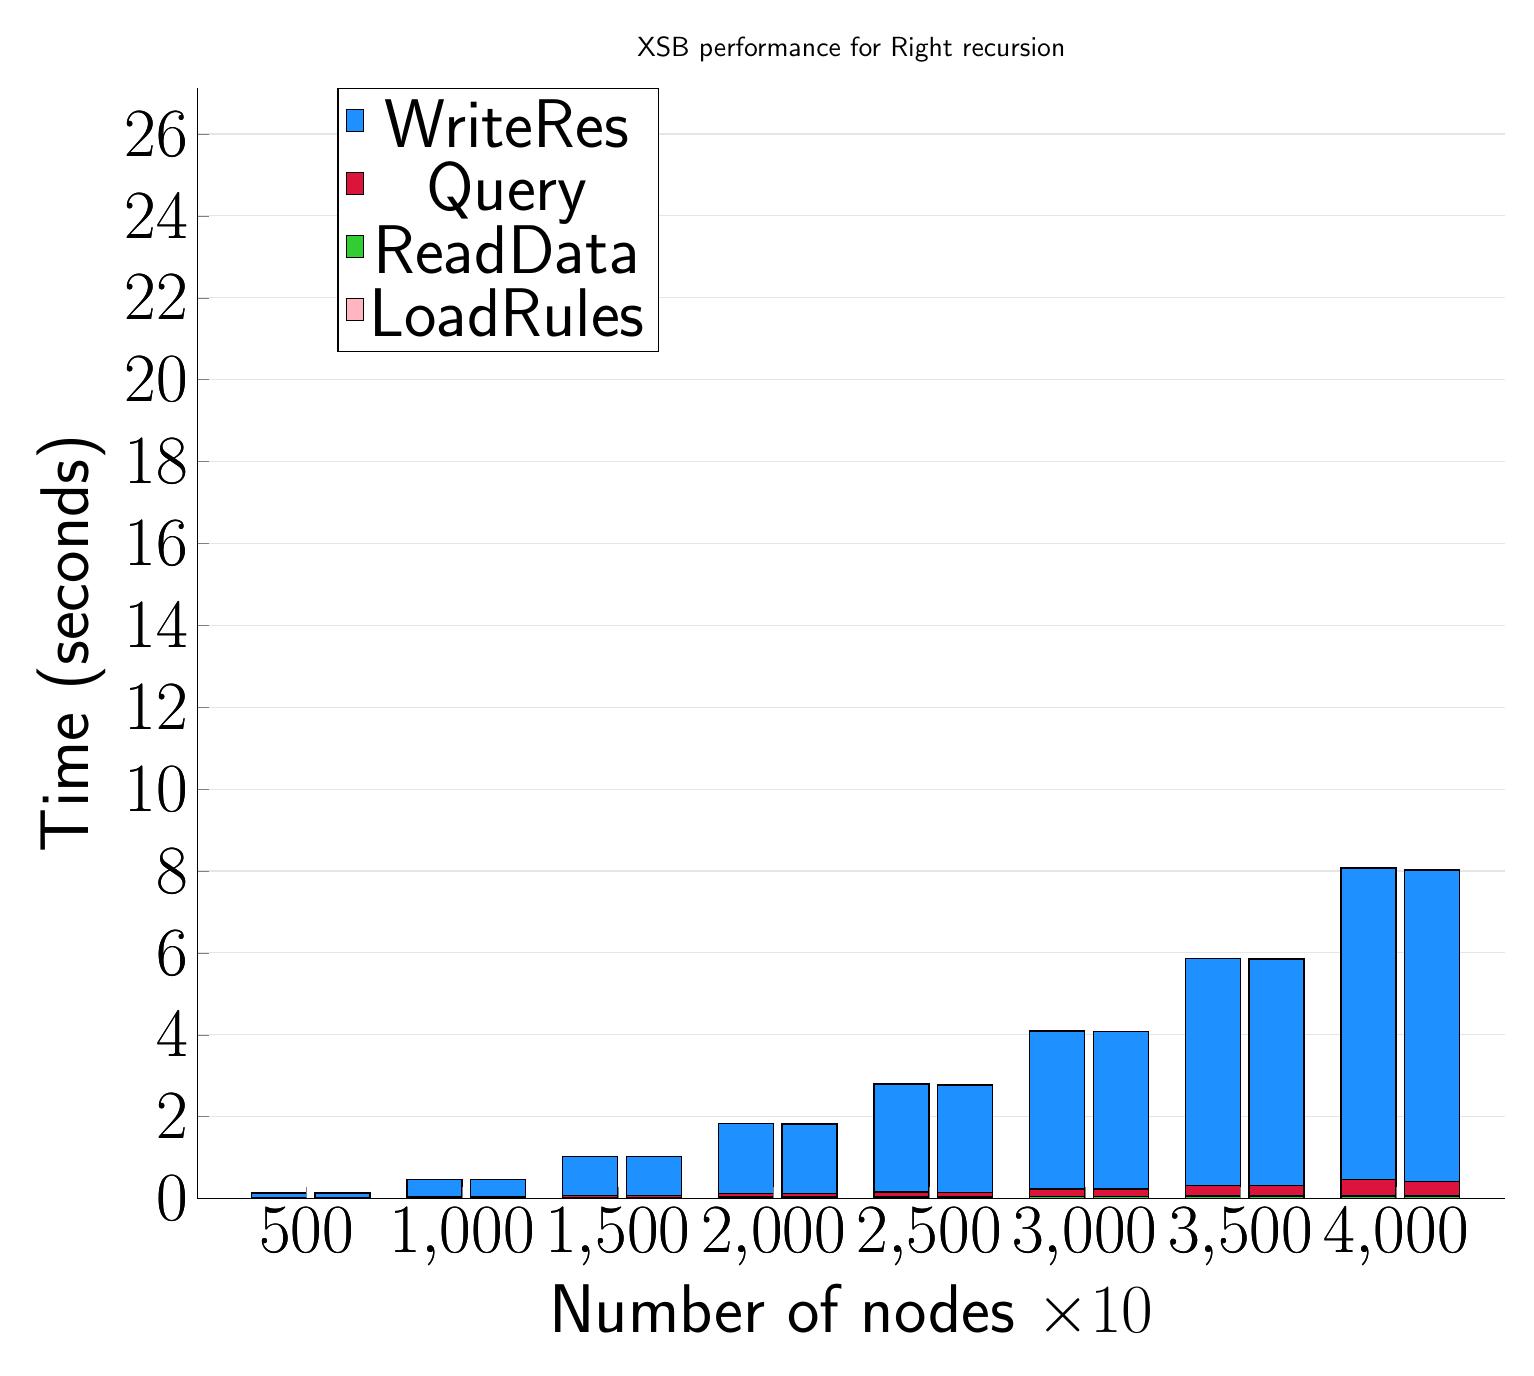
\begin{tikzpicture}
\begin{axis}[
   ybar stacked,
   title={XSB performance for Right recursion},
   bar shift=-10pt,
   width=1.5\textwidth,
   bar width=0.7cm,
   ymajorgrids, tick align=inside,
   major grid style={draw=gray!20},
   xtick=data,
   ymin=0, ymax=27.127176920572918,
   axis x line*=bottom,
   axis y line*=left,
   enlarge x limits=0.1,
   legend style={
       at={(0.23, 1)},
       anchor=north,
       legend columns=1,
       font=\Huge,
   },
   ylabel={Time (seconds)},
   xlabel={Number of nodes $\times 10$},
   label style={font=\Huge},
   tick label style={font=\Huge},
]
\addlegendimage{fill=DodgerBlue, draw=black, line width=0.2pt}
\addlegendentry{WriteRes}
\addlegendimage{fill=Crimson, draw=black, line width=0.2pt}
\addlegendentry{Query}
\addlegendimage{fill=LimeGreen, draw=black, line width=0.2pt}
\addlegendentry{ReadData}
\addlegendimage{fill=LightPink, draw=black, line width=0.2pt}
\addlegendentry{LoadRules}
\addplot +[fill=LightPink, draw=black, line width=0.5pt] coordinates {
    (500, 0.005634705225626626)
    (1000, 0.00475041071573893)
    (1500, 0.0049109458923339835)
    (2000, 0.004934628804524741)
    (2500, 0.0041209061940511065)
    (3000, 0.004262765248616536)
    (3500, 0.004485289255777993)
    (4000, 0.00468031565348307)
};
\addplot +[fill=LimeGreen, draw=black, line width=0.5pt] coordinates {
    (500, 0.010895331700642899)
    (1000, 0.0175299644470215)
    (1500, 0.024876038233439132)
    (2000, 0.03472733497619626)
    (2500, 0.0363407135009766)
    (3000, 0.0456542174021403)
    (3500, 0.05443572998046873)
    (4000, 0.061904350916544594)
};
\addplot +[fill=Crimson, draw=black, line width=0.5pt] coordinates {
    (500, 0.005786259969075523)
    (1000, 0.020816326141357398)
    (1500, 0.05028096834818523)
    (2000, 0.08388034502665204)
    (2500, 0.116741339365641)
    (3000, 0.18840932846069333)
    (3500, 0.26587335268656404)
    (4000, 0.4007866382598877)
};
\addplot +[fill=DodgerBlue, draw=black, line width=0.5pt] coordinates {
    (500, 0.11497441927591949)
    (1000, 0.42443267504374194)
    (1500, 0.9506541093190517)
    (2000, 1.7083843549092614)
    (2500, 2.6377449830373156)
    (3000, 3.851521968841553)
    (3500, 5.54369266827901)
    (4000, 7.606164932250977)
};
\end{axis}
\begin{axis}[
   ybar stacked,
   bar shift=13pt,
   width=1.5\textwidth,
   bar width=0.7cm,
   ymajorgrids, tick align=inside,
   major grid style={draw=none},
   xtick=data,
   ymin=0, ymax=27.127176920572918,
   axis x line*=none,
   axis y line*=none,
   enlarge x limits=0.1,
   label style={font=\Huge},
   tick label style={font=\Huge},
]
\addplot +[fill=LightPink, draw=black, line width=0.5pt] coordinates {
    (500, 0.005625666666666663)
    (1000, 0.004343333333333334)
    (1500, 0.004122333333333336)
    (2000, 0.003326333333333332)
    (2500, 0.003980999999999997)
    (3000, 0.003608333333333333)
    (3500, 0.004462333333333333)
    (4000, 0.004628666666666666)
};
\addplot +[fill=LimeGreen, draw=black, line width=0.5pt] coordinates {
    (500, 0.010901)
    (1000, 0.01751633333333333)
    (1500, 0.024878333333333332)
    (2000, 0.032998)
    (2500, 0.034127333333333336)
    (3000, 0.04551966666666666)
    (3500, 0.05416666666666667)
    (4000, 0.061450666666666674)
};
\addplot +[fill=Crimson, draw=black, line width=0.5pt] coordinates {
    (500, 0.005789666666666663)
    (1000, 0.01785233333333333)
    (1500, 0.044966)
    (2000, 0.08348100000000001)
    (2500, 0.113638)
    (3000, 0.18485033333333334)
    (3500, 0.2631673333333333)
    (4000, 0.354875)
};
\addplot +[fill=DodgerBlue, draw=black, line width=0.5pt] coordinates {
    (500, 0.114004)
    (1000, 0.42601)
    (1500, 0.9508220000000001)
    (2000, 1.7054456666666666)
    (2500, 2.625192333333333)
    (3000, 3.849727333333334)
    (3500, 5.526930666666666)
    (4000, 7.604004666666666)
};
\end{axis}
\end{tikzpicture}

\end{document}
